\section{Evaluation}
Our evaluation would take the form of a case study in which we would compare different approaches to testing the {\tt function checkRows()} is Sample Code \ref{dom0}, and measure how much coverage each approach can achieve.
The 3 approaches being compared are:
\begin{compactitem}
\item {\em Without HTML}
\item {\em Existing HTML} from the application
\item \tool generated HTML
\end{compactitem}

For each approach, we would follow the same methodology of loading and execution the function:
\begin{compactitem}
\item Load the target URL
\item Load the HTML (for that load HTML)
\item Execute the target code
\item Measure coverage
\end{compactitem}
Recalling from the Implementation section, the 4 steps above are identical to the initial 4 steps that our concolic driver would take in each iteration.  Additionally the concolic driver would take the executed paths as feedback and generate new HTML.  
For {\tt function checkRows()}, we can simply call the function via {\tt checkRows()} because it does not take any input arguments.

\begin{figure*}[ht]
\centerline{\scalebox{0.32}{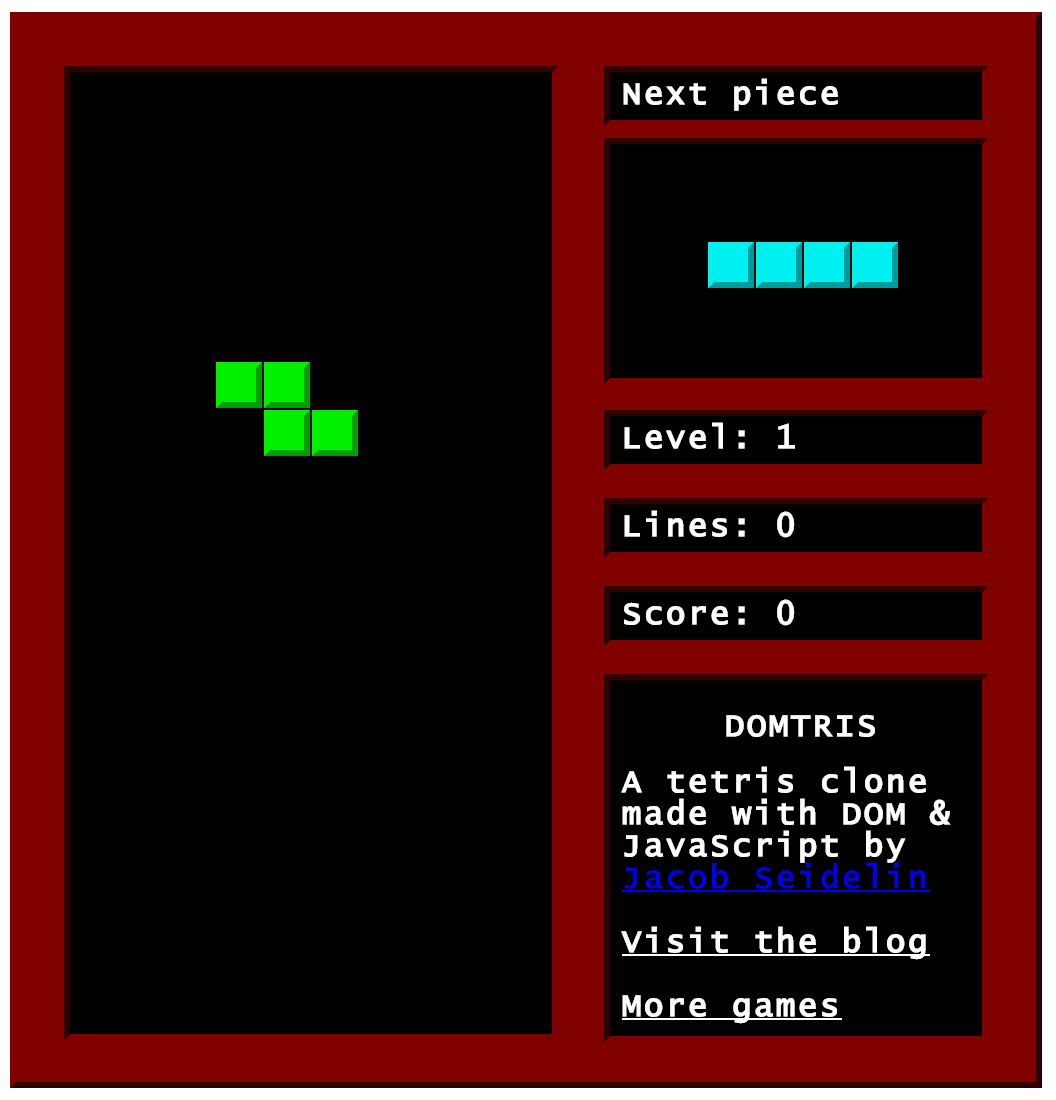
\includegraphics[natwidth=1056,natheight=1100]{domtris.png}}}
\caption[DOMtris game field]{The DOMtris game field (left) has 20 rows; thus {\tt field.children.length} should be 20 in our evaluation.}
\label{domtrisfield}
\end{figure*}

\begin{figure}[h]
\centerline{
\begin{tabular}{*2l|*3c}
\hline
& & \multicolumn{3}{c}{Count (Number Of)} \\ 
App & Function & Statements & Branches & Paths \\ \hline
DOMtris & checkRows() & 6 & 4 & 41 \\ \hline
\end{tabular}
}
\caption{Number of Statements, Branches and Paths of function being evaluated.}
\label{paths}
\end{figure}

\header{Counting Execution Paths.}
Figure \ref{paths} shows the number of statements, branches and paths that the function has.   
When counting the number of paths in the {\tt function checkRows()} in Sample Code \ref{dom0}, 
the original code does not pose an upper bound to the number of times the {\tt for} loop would get iterated because {\tt field.children.length} can be any value.
Therefore, we would set {\tt field.children.length} to a specific number for calculating the total number of possible execution paths in the function.
{\tt field} is set to have 20 children because the actual application always has 20 rows (Figure \ref{domtrisfield}). 
The following shows how the number of statements, branches and paths are counted for the {\tt function checkRows()}:
\begin{compactitem}
\item {\em Statements}: 6, {\tt line 2} to {\tt line 7}, inclusive.
\item {\em Branches}: 2 + 2. The {\tt for} loop has 2 branches: {\tt stay} and {\tt break}; plus the {\tt if} condition also has 2 branches: {\tt true} and {\tt false}. 
\item {\em Paths}: 20 ({\tt stay} branch in for loop) * 2 ({\tt true} and {\tt false} branches in {\tt if} statement) + 1 ({\tt break} branch).
\end{compactitem}

\begin{figure}[h]
\centerline{
\begin{tabular}{l|*3c}
\hline
& \multicolumn{3}{c}{Count (Number Of)} \\	
Approach & Statements & Branches & Paths \\ \hline
{\em Without HTML} & 0 & 0 & 0 \\ 
{\em Existing HTML} & 5 & 3 & 1 \\ 
\tool & 6 & 4 & 41 \\ \hline
\end{tabular}
}
\caption{Statement, Branch and Path coverage of different approaches to testing the {\tt function checkRows()}.}
\label{coverage}
\end{figure}

\header{Coverage Results.}
Figure \ref{coverage} shows the coverage results of different approaches to testing the {\tt function checkRows()}.  

The {\em Without HTML} approach cannot cover any statement because the first statement in the {\tt function checkRows()} is already a DOM operation requiring the existence of an element with {\tt id} {\tt "field"}.

The {\em Existing HTML} approach is able to cover 5 statements inclusively from {\tt line 2} to {\tt line 6} because the original HTML already has 20 rows inside {\tt field}.  
However the {\em Existing HTML} approach cannot cover the statement in {\tt line 7} because the rows do not have any children at the start of the game. 
{\em Existing HTML} is able to cover 3 of the 4 possible branches: both the {\tt stay} and {\tt break} branches in the {\tt for} loop, and the {\tt false} branch in the {\tt if} condition.  

% yahoo
% Tinysort
%  http://tinysort.sjeiti.com/
% Zen Coding
%  http://zen.sjeiti.com/
% DOMtris
%  http://www.ugrad.cs.ubc.ca/~k5r4/nbpAFZyrx5o/tracing/domtris/domtris.html
% Tudu
%  http://app.rasc.ch/tudu/welcome.action
% Knockout:
%  http://knockoutjs.com/examples/ 
% JQuery Widget: 
%  http://jqueryui.com/demos/
%  http://wijmo.com/widgets/
% Tizen
%   https://developer.tizen.org/downloads/sample-web-applications
%			mancala
